\documentclass{beamer}
\mode<presentation>
{
	\usetheme{Boadilla}
	\usecolortheme{dolphin}
	\usefonttheme{structureitalicserif}  % or try serif, structurebold, ...
	\setbeamertemplate{navigation symbols}{}
	\setbeamertemplate{caption}[numbered]
} 

\newcommand{\bul}{{\color{structure}\textbullet}}
\newcommand{\drawsquare}[3]{
    \draw (#1 - 0.5*#3, #2 - 0.5*#3) rectangle ++(#3, #3);
}


%\usepackage[utf8x]{inputenc}
\usepackage[T1]{fontenc}
\usepackage{csquotes}
\usepackage{comment}
\usepackage{amsmath}
\usepackage{enumerate}
\usepackage{graphicx}
\usepackage[colorinlistoftodos]{todonotes}
\usepackage{amssymb}
\usepackage{amsthm}
\usepackage{dsfont}
\usepackage{url}
\usepackage{color}
\usepackage{mathrsfs}
\usepackage{graphicx,wrapfig,lipsum}
\usepackage{verbatim}
\usepackage{dsfont}
\usepackage{bm}
\usepackage[backend=biber,style=numeric]{biblatex}
%%%%%%%%%%%%%%%%%%%%%%%%%%%%%%%%%%%%%%%%%%%%%%%%%%%%%%%%%%%%%%%%%%%%%%%%
%%% Preamble: Additional Packages
\usepackage{pdfpages}
%\usepackage{epigraph}
\usepackage{amsmath,amssymb}    % \mathcal{} = Calligraphy
\usepackage{amsfonts}           % \mathfrak{} = Fractur
\usepackage{amsthm}             % \mathbb{} = Blackboard font
\usepackage{verbatim}
\usepackage{subcaption}
%\usepackage{hyperref}
\usepackage{url}
\usepackage[breaklinks=true]{hyperref}
\usepackage{bm}
\usepackage{tikz}
\usetikzlibrary{arrows.meta}
\usepackage{tkz-fct}
\usepackage{enumerate}
\usepackage{enumitem}
\usepackage{multicol}
\usepackage[normalem]{ulem}
\usepackage{mathrsfs}


\hypersetup{
    colorlinks,
    citecolor=black,
    filecolor=black,
    linkcolor=black,
    urlcolor=black
}
\usepackage{biblatex}
\usepackage[shortcuts]{extdash} % Apparently this must be added *last*


\addbibresource{refs.bib}
% Required to come after \usepackage{biblatex}, so we include it here

% Load additional commands
\input{tex/preamble_commands_pres.tex}
%%%%%%%%%%%Operators necessary for the document%%%%%%%%%%%%%%%

\DeclareMathOperator*{\esssup}{ess\,sup}
\DeclareMathOperator*{\essinf}{ess\,inf}
\DeclareMathOperator*{\osc}{osc}
\DeclareMathOperator*{\supp}{supp}
\DeclareMathOperator*{\meas}{meas}



\addbibresource{refs.bib}
\title[New Korn Inequalities]{\huge{New Korn Inequalities and Applications to Fracture of Plates}}
\author[Andre]{André Martins Rodrigues \\ Advisor:Davit Harutyunyan}
\institute[UCSB]{University of California Santa Barbara}			
\date{19 of October, 2023}

\usebackgroundtemplate%
{%
	\includegraphics[width=\paperwidth,height=\paperheight]{figures/ucsb2}%
}
\setlength {\marginparwidth }{2cm}
\begin{document}
\begin{frame}[plain]
	\titlepage
\end{frame}
\begin{frame}[plain]
	\frametitle{Summary}
	\tableofcontents
\end{frame}


%\title{Revisiting the }
%\author{Andre Martins Rodrigues (University of California Santa Barbara)}

%\institute{SIAM, MS21, May 17-28, 2021}

%\date{\empty}
\section{Hyperelastic Bodies}
\begin{frame}{Hyperelastic Bodies}
    \begin{itemize}
        \item[\bul] Let $\Omega\subset\mathbb{R}^3$ be a bounded, set with a Lipschitz boundary.
        \vfill
        \item[\bul] Let $\Omega^\By$ the deformed state represented by $\By (\Bx) = \Bu(\Bx) + \Bx$
    \end{itemize}    
    \begin{figure}
        \includegraphics[scale=1]{figures/rigid.png}
    \end{figure}
    \end{frame}
    
    \begin{frame}{Hyperelastic Bodies}
    \begin{itemize}
        \item[\bul] If we add constraints to a body it will deform in a way that minimizes their energy.
        \vfill
        \item[\bul] The minimizer might not be unique since we can always add a rigid motion to the deformation.
        \vfill\pause
        \item[\bul] The  first strain energy density function, was called Green-St Venant strain tensor:
        \vl{\begin{equation*}
            W(\nabla \Bu) = \frac{1}{2}(\BC-I)=\frac{1}{2}(\nabla \Bu^T+\nabla \Bu + \nabla \Bu^T\nabla \Bu)
        \end{equation*}}
        \vfill\pause
        \item[\bul] The Linearized energy heavily depends on the symmetric gradient \vl{$e(\Bu)=\frac{1}{2}(\nabla \Bu+\nabla \Bu^T)$} and \vl{$\Bu= \By-\Bx$}.
    \end{itemize}
     %\item[\bul] Consider two close points in \vl{$\Bx, \Bx + \BGd \Bx $},  then applying Taylor expansion:
        %\vl{\begin{equation*}
        %|\By(\bm x + \delta \Bx)-\By(\Bx)|^2 = \delta \Bx^T \nabla \By^T(\Bx)\nabla \By(\Bx)\delta\Bx + o(\delta \Bx^2)
        %\end{equation*}}
        %\vfill
        %\item[\bul]  The symmetric tensor \vl{$ \BC:= \nabla \bm y^T(\bm x)\nabla \By(\Bx)$} is normally called in elasticity as the Cauchy-Green tensor.
        %\pause
        %\vspace{0.5cm}
        %\item[\bul] For a Rigid Motion \vl{$\By^r = a+R\Bx,\ a\in\R^3,\ R\in SO(3),$} the Cauchy-Green tensor is given by
        %\vl{\begin{equation*}\BC^r = R^TR = I.\end{equation*}}
    \end{frame}
    \begin{frame}
        \frametitle{Mathematical formulation: $3D$ hyperelasticity}
            
            We will work in the framework of $3D$ hyperelasticity. The Total energy of a deformation 
            {\color{violet}$y\colon \Omega\to\mathbb R^3$} of the body {\color{violet}$\Omega\subset\mathbb R^3$} is given by 
            {\color{violet}
            $$E(\boldsymbol{y})=\int_{\Omega} W(\nabla \boldsymbol{y(x)}) d x,
            $$
            }
            \pause
            The elastic energy density {\color{violet}$W\geq 0$} has the standard properties:
            \begin{itemize}
            \item[(i)] {\color{violet} $W(I)=0$} and {\color{violet} $W_F(I)=0$}. 
            
            \item[(ii)] Frame indifference: {\color{violet} $W(RF)=W(F)$} for every {\color{violet}$R\in SO(3).$}
            
            \item[(iii)] Local stability of the trivial deformation {\color{violet}$y(x)=x:$}\\
            \vspace{0.3cm}
            
            {\color{violet} $(L_0\xi,\xi)\geq \alpha|\xi|^2$} for some {\color{violet}$\alpha>0,$} and all {\color{violet}$\xi\in\mathrm{Sym}(\mathbb R^{3\times 3}).$}\\
            \item[(iv)] Non-degeneracy: {\color{violet}$\left(\mathrm{L}_{0} \xi,\xi\right)=0$} if and only if {\color{violet}$\xi^{T}=-\xi$}. 
            \vspace{0.3cm}
            Here, {\color{violet}$L_0=W_{FF}(I)$} is the linearly elastic stiffness tensor. 
            \end{itemize}
        \end{frame}
    \section{Imporance of Korn's Inequalities}
    \begin{frame}{Importance of Korn Inequality}
        \begin{itemize}
            \item[\bul]  Korn's first introduced this type of inequalities in 1906, to analysis of \vl{boundary value problems} in \vl{linear elasticity}. 
            \vfill\pause
            \item[\bul]  They help proving \vl{coercivity} of the bilinear form from variational formulation permitting to prove the \vl{existence of energy minimizers}.
        \end{itemize}
        \vfill\pause

        \begin{theorem}[First Korn Inequality] 
            Let \vl{$n \geq 3$,$1<p<\infty$}, and let the domain \vl{$\Omega \subset \mathbb{R}^n$} be open, bounded, connected, and Lipschitz.There there exists constants \vl{$C_1=C_1(\Omega,p)$} and \vl{$C_2=C_2(\Omega,p)$},such that for any vector field \vl{$\boldsymbol{u} \in W^{1,p}(\Omega:\R^n)$} there are \vl{$R\in\R^{n\times n}_{skw}$} such that:
            \vl{\begin{equation*}
               \label{eq:Korn1}
               \|\nabla \boldsymbol{u}-R\|_{L^p(\Omega)}^p \leq C_1\|e(\boldsymbol{u})\|_{L^p(\Omega)}^p .
               \end{equation*}}
           where \vl{$e(\boldsymbol{u})=\frac{1}{2}\left(\nabla \boldsymbol{u}+\nabla \boldsymbol{u}^T\right)$} is the symmetric part of the gradient. 
       \end{theorem}
    \end{frame}
    \begin{frame}{Buckling of Shells}
        \bul$\ $  The buckling load {\color{violet}$\lambda(h)$} is the smallest load for which this happens, so
{\color{violet}$$
\lambda(h)=\inf \left\{\lambda>0: \delta^{2} E_{tot}(\nabla y\phi ; h, \lambda)<0 \text { for some } \phi \in V_{h}\right\}
$$}\pause
{\color{violet}
$$
\hat{\lambda}(h)
=\inf_{\varphi} \left(-\frac{\int_{\Omega^h}(L_0e(\varphi),e(\varphi))dx}{\int_{\Omega^h}(\sigma_h,\nabla\varphi^T\nabla\varphi) dx}\right) 
$$}
\pause
        \begin{theorem}[{\color{purple} Grabovsky and Harutyunyan 2014}] Assume the conditions above are satisfied and 
            {\color{violet} $ \lim_{h\to 0} K^h(A)=0,$} where {\color{violet}$K^h(A)$} is the Korn constant of {\color{violet}$\Omega^h$} in {\color{violet}$A.$} If 
            {\color{violet} 
            $$
            \lim_{h\to 0} \frac{\hat{\lambda}(h)^2}{K^h(A)}=0,
            $$
            }
            then 
            {\color{violet} 
            $$
            \lim_{h\to 0} \frac{\lambda(h)}{\hat{\lambda}(h)}=1.
            $$
            }
        \end{theorem}
    \end{frame}
    \begin{frame}{Shell theory}
        \begin{itemize}
            \item[\bul] For general domains, the value of the Korn constant is not very important.
            \vfill
            \item[\bul] However, the rigidity of a shell \vl{$\Omega_h = S \times [-h, h]$} is closely related to the asymptotic of the optimal Korn's constants.
            \vfill\pause
            \item[\bul] The energy of a shell will always vanish with \vl{$h\to 0$}, but how fast?
            \\

                 Stretching - \vl{$E(\Bu_h)= h\ $}  Buckling -\vl{$E(\Bu_h)= h^2 \ $} Bending - \vl{$E(\Bu_h)= h^3$} 

            \vfill\pause
            \item[\bul] Most of the previous theories were based on $\Gamma$-convergence  of \vl{$ h^{-\alpha} E(\Bu_h)$} however this is not enough for \vl{$5/3\leq \alpha<2$}.
            %\vspace{0.5cm}
            \vfill\pause
            \item[\bul] Can we do it better with the right Korn's constant?
             %\vspace{0.5cm}
            \end{itemize}
        \end{frame}

\begin{frame}{Shell theory}
    Consider a minimizing sequence, \vl{$\Bu_h$} and its respective "normalization" \vl{$R_h$}.\pause For some $\alpha,\beta>0$ Let:
    \vl{\begin{equation*}
        \|e(\Bu)\|^2_{L^2(\Omega_h)}\sim E(\Bu_h)\sim h^\alpha\qquad K_1^2\sim \frac{1}{h^\beta}
    \end{equation*}}
    \pause
    Then for \vl{$\tilde{\Bu}_h= \Bu_h(x,y,\frac{1}{h})$} we have that:
    \vl{\begin{align*}
        \|\nabla \boldsymbol{\tilde{u}}_h-\tilde{R}_h\|^p_{L^p(\Omega_1)}&= \frac{C}{h}\|\nabla \boldsymbol{u}_h-R_h\|^p_{L^p(\Omega_h)}\\
        \pause
        &\leq \frac{C}{h^{\beta+1}}\|e(\Bu)\|^p_{L^p(\Omega_h)}\\
        &\leq C h^{\alpha-\beta-1}.
    \end{align*}}

    \bul$\ $ So to obtain the existence of minimizers we need \vl{$\beta\leq\alpha-1$}.
\end{frame}
\begin{frame}{Korn Inequalities in Shells}
    \begin{theorem}[Harutyunyan, Grabovsky  2014/2017/2018, H. and A.  2022 ]
        Let $K_{G},\kappa_{\theta}$ and $\kappa_{z}$ be the Gaussian curvature and the principal curvatures of the mid-surface $S$. Then then there exists a constant $C>0$ such that for all $h \in(0,1)$
        \begin{itemize}
            \item[\bul] If {$K_{G}>0$}, 
            \vspace{-0.2cm}
            {$$\|\nabla \boldsymbol{u}\|^{2} \leq \frac{C}{h}\|e(\boldsymbol{u})\|^{2}$$}
            \vspace{-0.8cm}
            \item[\bul] If {$K_{G}<0$},
            { $$
            \|\nabla \boldsymbol{u}\|^{2} \leq \frac{C}{h^{4 / 3}}\|e(\boldsymbol{u})\|^{2}$$}
            \vspace{-0.8cm}
            \item[\bul] If \vl{$k_z=k_\theta=0$} in an open set
            \vspace{-0.4cm}
            {\color{violet} $$
            \|\nabla \boldsymbol{u}\|^{2} \leq \frac{C}{h^2}\|e(\boldsymbol{u})\|^{2}$$}
            \vspace{-0.8cm}
            \item[\bul] If $k_z=0$ and $k_\theta>0$
            \vspace{-0.4cm}
            {
            $$
            \|\nabla \boldsymbol{u}\|^{2} \leq \frac{C}{h^{3/2}}\|e(\boldsymbol{u})\|^{2}$$}
            \vspace{-0.8cm}
            \item[\bul] If \vl{$k_z=0$} and \vl{$k_\theta\geq0$} and \vl{$k_\theta=0$} at finitely many points
            \vspace{-0.4cm}
            {\color{violet} 
            $$
            \|\nabla \boldsymbol{u}\|^{2} \leq \frac{C}{h^{12/7}}\|e(\boldsymbol{u})\|^{2}$$}
        \end{itemize}
    \end{theorem}   
\end{frame}
\section{Fracture Mechanics}
\begin{frame}{Fracture Mechanics}
    \begin{itemize}
        \item[\bul] The first mathematical model for the fracture of materials was proposed by Griffith in 1921.\vfill
        \item[\bul] It was already an energy model, however, there weren't enough mathematical tools to study it.
         \vfill   
        \item[\bul] Extending the approach from elasticity  has two main challenges:
        \pause
        \begin{itemize}
            \item[(i)]  We need to reconsider the space of admissible deformations; since Sobolev functions do not allow discontinuities.\pause
            \item[(ii)] We need to take into account that it takes energy to create and expand the crack.
        \end{itemize}
    \end{itemize}
    \begin{figure}
        \includegraphics{figures/crack2.png}
    \end{figure}
\end{frame}
\begin{frame}{Crack Energy}
\bul $\ $ Assuming that the crack is a hypersurface \vl{$\Gamma$} with finite \vl{$2$} Haussdorff measure, we can define the crack energy as: 
\vl{\begin{equation*}
    E_s(\Bu)=\int_{\Gamma} k(\Bx)  d\mathcal{H}^{2}(\Bx),
\end{equation*}}
\vfill
\bul $\ $ The first approach tried to understand the crack and the deformation \vl{$\Bu$} separately.
\vfill\pause

\bul $\ $ So let the crack be the jump set  of \vl{$\Bu$} and \vl{$k(\Bx)$} constant, we achieved the so-called Griffith's Energy:
\vl{$$E(\Bu) = \int_{\Omega\backslash J_\Bu} |e(\Bu)|^2dx + k\CH^2(J_\Bu)$$}
\vfill\pause
\textbf{Question:} For wich type of deformation $\Bu$ this energy make sense? Will still have a minimizer in that space?
\end{frame}
\section{Functions of Bounded Deformation}
\begin{frame}{Bounded Variation}
        \begin{definition}[BV Structure Theorem] A function \vl{$\Bu \in BV(\Omega)$} iff there exist a signed Radon measure \vl{$\mu$} on \vl{$\Omega$}  such that for all \vl{$\phi \in C_c^1\left(\Omega ; \mathbb{R}^n\right)$}, we have
            \vl{$$
        \int_\Omega \Bu \operatorname{div} \phi d x=-\int_\Omega \phi d\mu
        $$}
        So the weak derivative is a signed Radon measure and \vl{$D \Bu:=\mu.$}
        \end{definition}
        \pause
        \begin{center}
        \begin{figure}
            \begin{minipage}[b!]{0.48\textwidth}
                \includegraphics[scale=0.4]{figures/heavyside.png}
            \end{minipage}
            \pause
            \begin{minipage}[b!]{0.48\textwidth}
                \vspace{0.32cm}
                \includegraphics[scale=0.3]{figures/delta.png}
            \end{minipage}
            \end{figure}
        \end{center}
    \end{frame}
\begin{frame}{Bounded Deformation}
    \begin{definition}[Bounded Deformation Function \vl{$BD(\Omega$)}]
        Let $\Omega\subset\R^n$ and \vl{$\Bu=(u_1,u_2,\ldots,u_n) \in L^1(\Omega;\R^n)$}. Then, $\Bu$ is a function of bounded deformation in $\Omega$ if  the symmetric part of the distributional gradient of $\Bu$,i.e.:
        \vl{$$E_{ij}\Bu:=\frac{1}{2}(D_{i} u_j+D_ju_i) $$}
        is a \vl{Radon measure} with bounded total variation in $\Omega$ for any $i,j=1,\ldots,n$.
        \pause
        Additionally, this is a Banach space for the norm
        \vl{$$\|\Bu\|_{BD(\Omega)} = \|\Bu\|_{L^1(\Omega)}+\sum_{i,j}|E_{ij}\Bu|(\Omega)$$}
    \end{definition} 
  

\end{frame}
\begin{comment}
\begin{frame}{Bounded Deformation}
    \begin{theorem}[Bounded Deformation Function $BD(\Omega$)]
        For every \vl{$\BGx=\left(\xi_1, \ldots, \xi_n\right) \in \mathbb{R}^n$}, let $D_{\BGx}$ be the distributional derivative in the direction $\BGx$  and  \vl{$u^{\BGx}: \Omega \rightarrow \mathbb{R}$} defined by \vl{$$D_{\BGx} v=\sum_j \xi_j D_j v \qquad u^{\BGx}(\Bx)=(\Bu(\Bx), \BGx) $$}
         Then, for \vl{$\Bu\in L^1(\Omega)$,  $\Bu \in B D(\Omega)$} if 
         \vl{$$
        D_{\BGx} u^{\BGx}=(E \Bu \BGx , \BGx)
        $$}
        is a \vl{bounded Radon measure} on $\Omega$ for every $\BGx$ of the form \vl{$\Be_i+\Be_j,$} for   $i, j=1, \ldots, n$.
        \\
        \pause
         Conversely, if \vl{$\Bu \in B D(\Omega)$}, then \vl{$D_{\BGx} u^{\BGx}$ is a bounded Radon measure} on $\Omega$ for every $\BGx \in \mathbb{R}^n$.
    \end{theorem}
    
\end{frame}
\end{comment}

\begin{frame}{Jump Characterization}
    \bul$\ $  For real value functions, the jump set can be considered as the set where \vl{$\lambda(\Bx)= \operatorname{ap\ }\limsup _{\By \rightarrow \Bx} u(\By)$} and \vl{$\mu(\Bx) = \operatorname{ap\ }\liminf _{\By \rightarrow \Bx} u(\By)=\lambda(\Bx)$} are different.
    \vl{$$
    J_u:=\left\{\Bx \in \mathbb{R}^n \mid \lambda(\Bx)<\mu(\Bx)\right\},
    $$}
    \begin{figure}
        \includegraphics[scale=0.6]{figures/2dJump.png}
    \end{figure}
    \pause
    \bul$\ $ In the case of vector-valued functions we need to consider all the directions in which the jump can occur, \textit{i.e.}
    \vl{$$J_\Bu:=\{\Bu_{\BGv}^+(\Bx),\Bu_{\BGv}^-(\Bx)\ \text{exist and }  \Bu_{\BGv}^+(\Bx)\neq\Bu_{\BGv}^-(\Bx),\ \text{for some } \BGv\in S^{n-1}\}$$}
    where $\Bu_{\BGv}^\pm(\Bx)$ are the one-side Lebesgue limit in the direction $\BGv$. 
    %and they exist if:
    %\vl{$$\lim _{r \rightarrow 0^{+}} \frac{1}{r^n} \int_{B_r\left(\Bx\right)\cap H^\pm_{\BGv}}\left|\Bu(\By)-\Bu_{\BGv}^{\pm}(\Bx)\right| d \By=0.$$}
\end{frame}
\begin{frame}{Jump Characterization}
    \bul $\ $ If \vl{$\Bx \in J_\Bu$} then \vl{$\Bx$} is not Lebesgue so $$\vl{$ \CL^n(J_\Bu)=0.$}$$
    \pause\vfill
    \begin{theorem}[\vl{$\CH^{n-1}$} a.e. rectifiable] Let $\Bu\in BV(\Omega)$ or $\Bu\in BD(\Omega)$, then there exist countably many \vl{$C^1$-hypersurfaces}, $\left\{M_k\right\}_{k=1}^{\infty}$, such that
        \vl{$$
        \mathcal{H}^{n-1}\left(J_\Bu-\bigcup_{k=1}^{\infty} M_k\right)=0.
        $$}
        Additionally for each $M_k$ we have a unique $C^1$ outer vector $\BGv^k$ such that
        \vl{$$\BGv_\Bu(\Bx)=\BGv^k (\Bx),\quad \Bx\in M_k,$$}
        and  $\BGv_\Bu(\Bx)$ is  $\CH^{n-1} a.e.$ continuous  in $J_\Bu$ 
    \end{theorem}  
\end{frame}
\begin{frame}{Lebesgue Decomposition}
    \begin{definition} Let $\Bu \in B D(\Omega)$. Then we can decompose the vector value Randon measure $E\Bu$ into three parts:
        \vl{$$E \Bu=\CE \Bu \mathscr{L}^n + E_s \Bu\left\llcorner J_\Bu +E_c \Bu\right.$$}
        \pause
        Moreover, from the previous theorem, the jump part $E_j$ can be written as:
        \vl{$$E_J \Bu :=\left[ \left(\Bu_{\BGv_\Bu}^{+}-\Bu_{\BGv_\Bu}^{-}\right) \odot \BGv_\Bu\right] \mathscr{H}^{n-1}\left\llcorner J_\Bu\right.$$}
        \end{definition}
\pause\vfill
\bul $\ $ Additionally we say that \vl{$\Bu\in SBD(\Omega)$} if \vl{$E_c\Bu = 0$}, so for $\Bu\in SBD(\Omega)$ we have:
\vl{$$ \int_{\Omega\backslash J_\Bu} |e(\Bu)|^2dx + k\CH(J_\Bu)\approx \int_\Omega E\Bu $$}
\end{frame}
\begin{frame}{Important Properties and Korn Inequality}
    \begin{itemize}
        \hspace{1cm}
        \begin{columns}
            \begin{column}{0.3\textwidth}  % Adjusting the width to less than 0.5 to leave some space between columns
                \item[\bul] Lower semicontinuity
                 \vfill
                \item[\bul] Sobolev embedding
            \end{column}
            \begin{column}{0.65\textwidth}
                \item[\bul] Existence of Trace and Extension Results
                \vfill
                \item[\bul] Poincare inequality
            \end{column}
        \end{columns}
    \end{itemize}
    \vfill\pause
    \begin{theorem}\label{KornBDGeneralDomain}
        Let $n \in \mathbb{N}$ with $n \geq 2, p \in(1, \infty)$, and let $\Omega \subset \mathbb{R}^n$ be a bounded connected and open Lipschitz set. There exists $c=c(n, p, \Omega)>0$ such that, for any $\Bu \in$ $ S B D^p(\Omega)$, there is a set of \vl{finite perimeter $\omega \subset \Omega$} with \vl{$\mathcal{H}^{n-1}\left(\partial^* \omega\right) \leq c \mathcal{H}^{n-1}\left(J_u\right)$} and a skew-symmetric matrix R such that
        \vl{$$
        \int_{\Omega\backslash\omega}|\nabla \Bu-R|^p dx \leq c(n, p, \Omega) \int_{\Omega} |e(\Bu)|^p dx
        $$}
        The constant $c$ is invariant under uniform scalings of the domain.
    \end{theorem}
\end{frame}
\section{Korn inequality for plates  of \vl{$SBD$} functions} 
\begin{frame}{Korn Inequality in plates for SBD}
    \begin{theorem}[A. 2023] Let $D=[-1,1]^2$ and $\Omega_h = D\times[-h,h]$ for some small $h$. Then for $\delta>0$ small enough, there exists $C = C(p)>0$, such that for any $\Bu\in SBD^p(\Omega_h)$ with \vl{$\CH^2(J_u)<\delta h$} there is a set $\omega\in\Omega_h$ with \vl{$\CL^3(\omega)\leq C \CH^2(J_u)$}  and a skew-symmetric matrix $A$ such that
        \vl{$$\|\nabla \Bu-R\|^p_{L^p(\Omega_h \backslash \omega)} dx \leq \frac{C(p)}{h^p} \|e(\Bu)\|^p_{L^p(\Omega_h)}$$}
    \end{theorem}
\end{frame}
\begin{frame}{Korn inequality in plates for Sobolev functions, revisited}
    $$\text{Goal:} \textcolor{violet}{
        \int_{\Omega_h}|\nabla \Bu-R|^p dx \leq \frac{c(n, p, \Omega)}{h^p} \int_{\Omega_h} |e(\Bu)|^p dx
    }$$\pause
  \begin{minipage}{0.4\textwidth}
    \begin{figure}
        \includegraphics[scale=0.3]{figures/plate.png}
    \end{figure}
\end{minipage}
\begin{minipage}{0.58\textwidth}
    \begin{itemize}
        \item[1.] Split the plate in \vl{$N^2$} overlapping cubes of size \vl{$Ch^3$}.
        \vfill\pause
        \item[2.] Apply  Korn inequality in each cube to obtain skew-symmetric matrices \vl{$R_{i,j}$}.
        \vfill
    \end{itemize}
\end{minipage}
\begin{itemize}
        \item[3.] Interpolate the matrices \vl{$R_{i,j}$} to obtain a piecewise function $R_h$.
        \vfill
        \item[4.] Apply Poincaré inequality to \vl{$R_h$} to obtain constant matrix \vl{$R_*$}.
        \vfill
        \item[5.] Choose the closest skew-symmetric matrix to \vl{$R_*$} to obtain the desired matrix \vl{$R$}.
    \end{itemize}

\end{frame}
\begin{frame}{ Korn inequality in plates for Sobolev, new proof}
    
    \begin{itemize}[leftmargin = 1.5cm]
     \item[Step 1:] Let \vl{$N:= \frac{1}{h}$}, split $\Omega_h$ in \vl{$(N-1)^2$}  overlapping cubes of size \vl{$(2h)^3$} and apply the general Korn inequality in each one
     \vl{$$\|\nabla \Bu- R_{i,j}\|_{L^p(D_{i,j})} \leq C_0(p) \|e(\Bu)\|_{L^p(D_{i,j})}$$}
    \vfill\pause
    \item[Step 2:] For 2 intersecting cubes \vl{$D_{i,j}$} and \vl{$D_{i',j'}$}, by triangular inequality we can bound the difference of the matrices as:
    \vl{$$ (2h)^3|R_{i,j}-R_{i',j'}|^p\leq C(p) \left(\|e(\Bu)\|^p_{L^p(D_{i,j})}+\|e(\Bu)\|^p_{L^p(D_{i',j'})}\right).$$}
    \end{itemize}
\end{frame}
\begin{frame}{ Korn inequality in plates for Sobolev, new proof}
    \begin{itemize}[leftmargin = 1.5cm]
        \item[Step 3:]Fix a cube in the first collum, $j=1$, and for any cube $D_{k,L}$ we can consider the path of order \vl{$\CO(N)$}:
        \input{figures/grid1Presentation.tex}
        
    \end{itemize}
    \begin{align*}
        \|\nabla u- R_{i,1}\|^p_{L^p(D_{k,l})} &= \left\|\nabla \Bu+ \sum_{(j,m)\text{ in Path}}^l (R_{j,m}-R_{j',m'})-R_{k,l}\right\|^p_{L^p(D_{k,l})}
        \\
        &\leq C(p)  \textcolor{violet}{N^{p-1}}\left(\|e(\Bu)\|^p_{L^p(D_{i,-})}+\|e(\Bu)\|^p_{L^p(D_{-,l})}\right).
        \end{align*}
\end{frame}
\begin{frame}{ Korn inequality in plates for Sobolev, new proof}
    \begin{itemize}[leftmargin = 1.5cm]
        \item[Step 4:] To get the result for $\Omega_h$ we can sum over all \vl{$(k,l)$} obtaining:
    \end{itemize}
    \begin{align*}
        \|\nabla \Bu- R_{i,1}\|^p_{\Omega_h}&\leq\sum_{k=1}^{N-1}\sum_{l=1}^{N-1}\|\nabla \Bu- R_{i,1}\|^p_{L^p(D_{k,l})}  \\
        &\leq C(p)\textcolor{violet}{N^{p-1}}\left(\textcolor{violet}{ N^2} \|e(\Bu)\|^p_{L^p(D_{i,-})} +  2\textcolor{violet}{N}\|e(\Bu)\|^p_{L^p(\Omega_h)}\right).
    \end{align*}
    \pause
    \begin{itemize}[leftmargin = 1.5cm]
        \item[Step 5:] To get the desired asymptotic we can sum of $i$:
    \end{itemize}
    \begin{align*}
        \sum_{i=1}^{N-1} \|\nabla \Bu - R_{i,1}\|^p_{L^p(\Omega_h)}&\leq C(p)\textcolor{violet}{N^{p+1}}\|e(\Bu)\|^p_{L^p(\Omega_h)}.
    \end{align*}
    \pause
    \begin{itemize}[leftmargin = 1.5cm]
        \item[Step 6:] Since we sum over \vl{$N-1$} elements there must be a $i'$ that satisfy the desired asymptotic.
    \end{itemize}
\end{frame}
\begin{frame}{Korn inequality for plates  of \vl{$SBD$} functions, proof}
    \begin{theorem} Let $D=[-1,1]^2$ and $\Omega_h = D\times[-h,h]$ for some small $h$. Then for $\delta>0$ small enough, there exists $C = C(p)>0$, such that for any $\Bu\in SBD^p(\Omega_h)$ with \vl{$\CH^2(J_u)<\delta h$} there is a set $\omega\in\Omega_h$ with \vl{$\CL^3(\omega)\leq C \CH^2(J_u)$}  and a skew-symmetric matrix $R$ such that
        \vl{$$\|\nabla \Bu-R\|^p_{L^p(\Omega_h \backslash \omega)} dx \leq \frac{C(p)}{h^p} \|e(\Bu)\|^p_{L^p(\Omega_h)}$$}
    \end{theorem}
    \pause
    \vfill
\begin{itemize}[leftmargin = 1.5cm]
    \item[Step 1:] Let $N:= \frac{1}{h}$, split $\Omega_h$ in $(N-1)^2$  overlapping cubes of size $(2h)^3$ and apply the general Korn inequality in each one:
    \begin{equation*}\label{kornkj}
    \|\nabla \Bu- R_{i,j}\|^p_{L^p(D_{i,j}\backslash \omega_{i,j})} \leq C_0(p) \|e(\Bu)\|^p_{L^p(D_{i,j})}.
    \end{equation*}
    with \vl{$\CH^2(\partial^*\omega_{i,j})\leq C \CH^2(J_u\cap D_{i,j})$} and by the isoperimetric \vl{$\CL(\omega_{i,j})\leq 2C_ph\CH^2(J_u\cap D_{i,j}).$}
\end{itemize}
\end{frame}
\begin{frame}{Korn inequality for plates  of $SBD$ functions, proof}
    \begin{itemize}[leftmargin = 1.5cm]
        \item[Step 2:] If a part of the jump lands on one cube we can't control the size of the matrices between cubes. So we can define a cube to be good when:
        \vl{$$\CH^2(J_u\cap D_{k,j})\leq \frac{1}{4C_pC_0} h^2, \quad \CL(\omega_{k,j})\leq h^3,$$}
    \pause
    Remark: \vl{$ \CH^0(B_{idx})\leq\frac{C\CH^2(J_u)}{h^2},\qquad
    \CH^0(B_{idx})\leq C \delta N.$}
    \pause\vfill
        \item[Step 4:] Let $D_{i,-}$ be a bad row if at has at least one bad cube, and similar to columns. Then we can construct $\omega$ as:
    \end{itemize}
        \vfill
        $$\omega = \left(\bigcup_{i\in B^r_{idx},j\in B^c_{idx}}D_{i,j}\right)\bigcup \left(\bigcup_{i,j} \omega_{i,j}\right)\qquad \textcolor{violet}{\CL(\omega)\leq C \delta \CH^2(J_u)}.$$
    \begin{itemize}[leftmargin= 1.5cm] 
        \vfill\pause
        \item And now on a good cube everything not in $\omega$.
    \end{itemize}
\end{frame}

\begin{frame}{Korn inequality for plates  of $SBD$ functions, proof}
\begin{itemize}[leftmargin = 1.5cm]
    \item[Step 5:] Fix a good cube in the first collum, $j=1$, and for any good cube $D_{k,L}$ we need to find a path of order \vl{$\CO(N)$}. Additionally, for any given cube outside row $i$ we need to make sure that there are no more than \vl{$\CO(N)$} paths passing by.
\end{itemize}
\input{figures/grid2Presentation.tex} 
\end{frame}
\section{Weighted Korn Inequalities}
\begin{frame}{Weighted Korn Inequality in Bulk Domains}
    \begin{theorem} [Weighted  Korn Inequality ]\label{KornGamma} Let $\Omega \subset \mathbb{R}^n$ be a connected, bounded $(L, R)$-Lipschitz set,  $\GG$ an nonempty  close subset of $\dOm$ and \vl{$\delta_\GG(\Bx)=\dist(\Bx, \partial\GG)$}. Then for any $\Bu \in W_{\mathrm{loc}}^{1, p}\left(\Omega ; \mathbb{R}^k\right)$, with $p \in(1, \infty)$, and every $\alpha\geq0$ there is are  $R \in \mathbb{R}_{\mathrm{skw}}^{n \times n}$ such that
        \vl{$$
        \|\delta_\GG(\Bx)^\alpha(\nabla \Bu-R)\|_{L^p(\Omega)} \leq  c(n,p,\alpha,L,R)\left\|\delta_\GG(\Bx)^\alpha e(\Bu)\right\|_{L^p(\Omega)}.
        $$}
    \end{theorem}
\pause
    \begin{itemize}
        \item[\bul] Useful when it's necessary the use opolar coordinates or other change of variables.
        \pause\vfill
        \item[\bul] Better control around the solid's boundary paves the way for localization techniques.
    \end{itemize}
    
\end{frame}
\begin{frame}{Weighed Poincare Inequality}
    \begin{theorem}[Weighted Poincaré Inequality] \label{WeightedPoincareOld} Let $\Omega \subset \mathbb{R}^n$ be a connected, bounded $(L, R)$-Lipschitz set,  $\GG$ an nonempty closed subset of $\dOm$  and \vl{$\delta_\GG(\Bx)=\dist(\Bx, \partial\GG)$}. Then for any $\Bu \in W_{\mathrm{loc}}^{1, p}\left(\Omega ; \mathbb{R}^k\right)$, with $p \in[1, \infty)$, and every $\alpha\geq 0$ there is $\Ba \in \mathbb{R}^k$ such that:
        \vl{$$
        \|\delta_\GG(\Bx)^\alpha (\Bu-\Ba)\|_{L^p(\Omega)} \leq c(n,p,\alpha,L,R)\|\Gd_\GG(\Bx)^{1+\Ga} \nabla \Bu\|_{L^p(\Omega)} .
        $$}
    \end{theorem}
    \vfill
    \bul$\ $ The techniques used will be similar to the ones we will use to prove the weighted Korn inequality in plates so we can skip for now.
\end{frame}
\begin{frame}{Weighted Korn Inequality, Proof} 
    \begin{itemize}[leftmargin = 1.5cm]
        \item[Step 1:]  Consider a Whitney Cover of $\Omega$:
        \begin{center}
            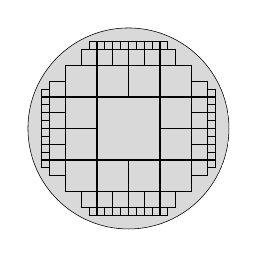
\begin{tikzpicture}[scale=0.8]
                % Drawing the circle
                \path[clip] (0,0) circle (1.6);
                \draw[fill=gray!30] (0,0) circle (1.6);
                
                \drawsquare{0}{0}{1}
                \draw (0.5,0.5) rectangle ++(0.5,0.5);
                \draw (0.5,0) rectangle ++(0.5,0.5);
                \draw (0.5,-0.5) rectangle ++(0.5,0.5);
                \draw (0.5,-1) rectangle ++(0.5,0.5);
        
                \draw (-1,0.5) rectangle ++(0.5,0.5);
                \draw (-1,0) rectangle ++(0.5,0.5);
                \draw (-1,-0.5) rectangle ++(0.5,0.5);
                \draw (-1,-1) rectangle ++(0.5,0.5);
        
                \draw (-0.5,-1) rectangle ++(0.5,0.5);
                \draw (0,-1) rectangle ++(0.5,0.5);
                \draw (-0.5,0.5) rectangle ++(0.5,0.5);
                \draw (0,0.5) rectangle ++(0.5,0.5);
                \foreach \i in {-0.75,-0.5,...,0.5}{
                    \draw(1,{\i}) rectangle ++(0.25,0.25);
                    \draw(-1.25,{\i}) rectangle ++(0.25,0.25);
                }
                \foreach \i in {-0.75,-0.5,...,0.5}{
                    \draw({\i},1) rectangle ++(0.25,0.25);
                    \draw({\i},-1.25) rectangle ++(0.25,0.25);
                }
                
                \foreach \i in {-0.625,-0.5,...,0.5}{
                    \draw(1.25,{\i}) rectangle ++(0.125,0.125);
                    \draw(-1.375,{\i}) rectangle ++(0.125,0.125);
                    \draw({\i},1.25) rectangle ++(0.125,0.125);
                    \draw({\i},-1.375) rectangle ++(0.125,0.125);
                }
            \end{tikzpicture}
        \end{center}
        \pause
        \vl{$$\sqrt{n} \ell\left(Q_j\right) \leq \operatorname{dist}\left(Q_j, \GG\right) \leq 4 \sqrt{n} \ell\left(Q_j\right).$$}
        \pause
        And then apply the normal Korn inequality in each cube to obtain:
        \begin{align*}    
            \left\|\delta_\GG(\Bx)^\alpha\nabla (\Bu-R_j)\right\|_{L^p(Q_j)} & \leq (4\sqrt{n} r_j)^\alpha \left\|\nabla (\Bu-R_j)\right\|_{L^p(Q_j)}\\ &\leq C (4\sqrt{n} r_j)^\alpha \left\|e(\Bu)\right\|_{L^p(Q_j)}\\
            &\leq C(n,p,\alpha)  \left\|\delta_\GG(\Bx)^\alpha e(\Bu)\right\|_{L^p(Q_j)}.
        \end{align*}
    \end{itemize}
        
\end{frame}
\begin{frame}{Weighted Korn Inequality, Proof}
\begin{itemize}[leftmargin = 1.5cm]\item[Step 2:] Construct a \vl{partition of unity} subordinated to this cover and interpolate the matrices $R_j$ to obtain a piecewise function 
\end{itemize}
$$\textcolor{violet}{\beta = \sum_j \varphi_j R_j,}\quad \|\delta_\GG(\Bx)^\alpha(\nabla \Bu-\beta)\|_{L^p(\Omega)}\leq  C(n,p) \left\|\delta_\GG(\Bx)^\alpha e(\Bu)\right\|_{L^p\left(\Omega\right)}.  $$
\begin{itemize}[leftmargin= 1.5cm]  
    \item[Step 3:] Since \vl{$ \delta_\GG(\Bx)\left|\nabla \varphi_j\right|(\Bx) \leq C \chi_{Q_j}(\Bx)\text { for all } \Bx \in \Omega$} and \vl{$\sum_j \nabla \varphi_j=0$} we can apply the weighted Poincare inequality to obtain $R_*$ such that:
    \pause
\end{itemize}
\begin{align*}
    \left\|\delta_\GG(\Bx)^{\alpha}(\beta-R_*)\right\|_{L^p(\Omega)} &\leq C \|\delta_\GG(\Bx)^{(1+\alpha) }\nabla \beta\|_{L^p(\Omega)}\\
    & \leq C \sum_j \|\delta_\GG(\Bx)^{(1+\alpha)}\nabla \varphi_j\left(\nabla \Bu-R_j\right)\|_{L^p(Q_j)} \\
    &\leq C(n,p,\alpha,L,R)\|\delta_\GG(\Bx)^{\alpha}e(\Bu)\|_{L^p(\Omega)}.
\end{align*}
\vfill\pause
\begin{itemize}[leftmargin = 1.5cm]
    \item[Step 4:] \vl{$R$ to be the closest skew symmetric matrix to $R_*$}.
\end{itemize}

\end{frame}
\begin{frame}{Weighted Korn inequality for plates}
\begin{theorem}[Weighted Korn Inequality and Uniform Rigidity for Plates] \label{KornGammaPlate} Let $\Omega_h=\Omega\times I_h \subset \mathbb{R}^3$ be a shell such that $\Omega$ is  a connected, bounded $(L, R)$-Lipschitz set and $I_h=[-h,h]$ for small $h>0$. Additionally, let \vl{$\delta'(\Bx)=\delta_{\dOm\times I_h}=\dist(\Bx,\dOm\times I_h)$} and $p \in(1, \infty)$. Then for any $\Bu \in W^{1, p}\left(\Omega_h ; \mathbb{R}^n\right)$ and any $\alpha\geq 0 $ , there  is $R \in \mathbb{R}_{\mathrm{skw}}^{3 \times 3}$ such that
    \vl{$$
        \|\delta'(\Bx)^\alpha(\nabla \Bu-R)\|_{L^p(\Omega)} \leq  \frac{c(n,p,\alpha,L,R)}{h}\left\|\delta'(\Bx)^\alpha e(\Bu)\right\|_{L^p(\Omega)}.
    $$}
\end{theorem}
\end{frame}
\begin{frame}{Weighted Korn inequality for plates, Proof}
%\begin{itemize}[leftmargin = 1.5cm]
%\end{itemize}

\begin{center}
    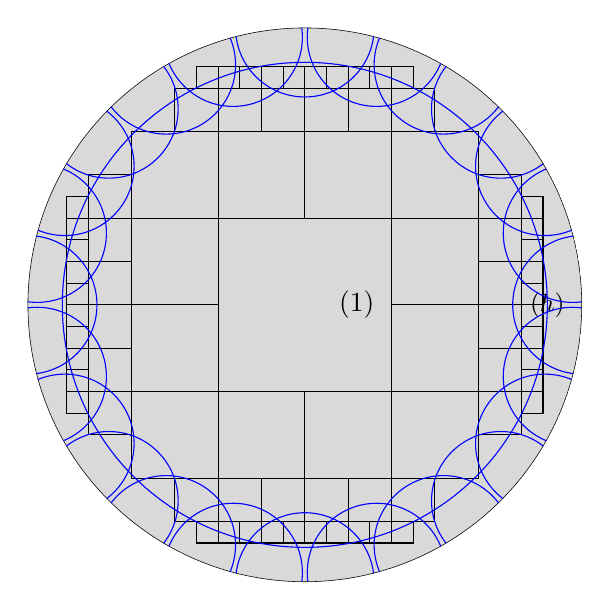
\begin{tikzpicture}[scale=2.2]
        % Drawing the circle
        \path[clip] (0,0) circle (1.6);
        \draw[fill=gray!30] (0,0) circle (1.6);
        
        % Drawing squares as part of the "Whitney cover"
     
    
        %\foreach \i in {22.5,67.5,...,337.5} {
            %\draw ({1.5*cos(\i)},{1.5*sin(\i)}) rectangle ++(0.4,0.4);
        %}
    
        % Drawing some squares towards the center
        %\draw (-0.5,-0.5) rectangle (0.5,0.5);
        \drawsquare{0}{0}{1}
        \draw (0.5,0.5) rectangle ++(0.5,0.5);
        \draw (0.5,0) rectangle ++(0.5,0.5);
        \draw (0.5,-0.5) rectangle ++(0.5,0.5);
        \draw (0.5,-1) rectangle ++(0.5,0.5);

        \draw (-1,0.5) rectangle ++(0.5,0.5);
        \draw (-1,0) rectangle ++(0.5,0.5);
        \draw (-1,-0.5) rectangle ++(0.5,0.5);
        \draw (-1,-1) rectangle ++(0.5,0.5);

        \draw (-0.5,-1) rectangle ++(0.5,0.5);
        \draw (0,-1) rectangle ++(0.5,0.5);
        \draw (-0.5,0.5) rectangle ++(0.5,0.5);
        \draw (0,0.5) rectangle ++(0.5,0.5);
        \foreach \i in {-0.75,-0.5,...,0.5}{
            \draw(1,{\i}) rectangle ++(0.25,0.25);
            \draw(-1.25,{\i}) rectangle ++(0.25,0.25);
        }
        \foreach \i in {-0.75,-0.5,...,0.5}{
            \draw({\i},1) rectangle ++(0.25,0.25);
            \draw({\i},-1.25) rectangle ++(0.25,0.25);
        }
        
        \foreach \i in {-0.625,-0.5,...,0.5}{
            \draw(1.25,{\i}) rectangle ++(0.125,0.125);
            \draw(-1.375,{\i}) rectangle ++(0.125,0.125);
            \draw({\i},1.25) rectangle ++(0.125,0.125);
            \draw({\i},-1.375) rectangle ++(0.125,0.125);
        }
        %write 1 at (0,0,5)
        \node at (0.3,0) {$\CO(1)$};
        \node at (1.4,0) {\small{$\CO(h)$}};
        \pause
        \draw[blue] (0,0) circle (1.4);
        \foreach \i in {0,15,...,345} {
            \draw[blue] ({1.6*cos(\i)},{1.6*sin(\i)}) circle (0.4);
        }
    \end{tikzpicture}
\end{center}

\end{frame}

%\begin{frame}{References}
%    \printbibliography
%\end{frame}
    
\end{document}   

    
    
    
    \section{Introduction to Buckling}
    \begin{frame}
     
    \frametitle{Axial Compression of the cylindrical shell}
    
    \vspace{-5cm}
    
    
    %\begin{figure}
    %\includegraphics[scale=0.5]{pic3.pdf}
    %\end{figure}
    
    \vspace{-6cm}
    
    
    A cylindrical shell of radius $R>0,$ height $L>0$ and thickness $h>0$ (a small parameter) given by  
    {\color{violet}
    $$\Omega^h=\{(r,\theta,z) \ : \ r\in[R-h/2,R+h/2], \ \theta\in [0,2\pi), \ z\in[0,L]\}$$
    }
    undergoes axial homogeneous compression.
    
    \end{frame}
    
    
    
    
    \begin{frame}
    \frametitle{Problem set up}
    \vspace{-0.5cm}
    %\begin{figure}
    %\includegraphics[scale=0.35]{Cylinder.1.pdf}
    %\end{figure}
    \vspace{-0.5cm}
    {\color{blue}\underline{Loading.}} The bottom rests on a flat substrate. The load {\color{violet} $t(x,\lambda)=-\lambda e_z$} will be applied at the top, where the magnitude  {\color{violet} $\lambda$} will be increased from zero continuously.  
    \end{frame}
    
    \begin{frame}
    
    \frametitle{The shell buckling}
    
    
    %\begin{figure}
    %\includegraphics[scale=0.32]{cylinderbuckling.png}
    %\end{figure}
    
    Assume the shell is made of an elastic material. Then the shell {\color{red}buckles} at some critical load {\color{red}$\lambda>0$,} 
    that depends on {\color{violet}R,L,h} and the material.
    
    %\pause
    {\color{blue}\underline{Goal:}} Derive an asymptotic formula for  {\color{red}$\lambda$}  as {\color{violet}$h\to 0.$} 
    \end{frame}
    \section{Previous results}
    
    \begin{frame}
    \frametitle{What is known?}
    
    {\color{blue}\underline{Deformation:}} Typically diamond-like shapes are formed on various parts of the shell (there may be only one).
    %\pause
    \vspace{0.8cm}
    
    {\color{blue}\underline{Koiter's formula (1945)}} (isotropic materials).  
    
    {\color{violet}
     $$\lambda =\frac{Eh}{R\sqrt{3(1-\nu^{2})}},$$
    }
    where {\color{violet}$E$} and {\color{violet}$\nu$} are the Young's modulus and the Poisson ratio, respectively.
     
    
    \vspace{0.8cm}
    
    {\color{blue}\underline{Remark}} 
    Although the formula was derived by {\color{purple}R. Lorenz (1911)} and independently by {\color{purple}S. Timoshenko (1914),}
    it is known as "Koiter's formula", as it seems to have been independently derived yet another time by Koiter in his Ph.D. thesis in 1945.
    
    
    \end{frame}
    
    
    
    \begin{frame}
    
    
    \frametitle{Experimental vs Theoretical results}
    
    
    {\color{red}\underline{Warning.}} Experiments have shown that in fact, the theoretical result (Koiter's formula) does not provide 
    an accurate value for the critical buckling load. In fact experimental observations show
    {\color{violet}
     $$\lambda(h) \sim h^{3/2}\qquad\text{as}\qquad h\to 0.$$
    }
    \vspace{-0.5cm}
    \begin{figure}
    \includegraphics[scale=0.6]{figures/experiments2.png}
    \caption{ Normalized buckling stress versus
    radius/thickness. The best fitting line has a slope of $-1.5$ while the theoretical value is $-1$,  \cite{Bucklingparadox} }
    \end{figure}
    
    \end{frame}
    
    
    \begin{frame}
    \frametitle{Experimental vs Theoretical results}
    This is believed to be due to the {\color{blue}imperfections} (of the shell or the load). 
    
    \vspace{0.3cm}
    
    This phenomenon is called {\color{red}sensitivity to imperfections.}  
    
    \vspace{0.3cm}
    
    %\pause
    {\color{blue}\underline{Our task.}} 
    \begin{itemize}
    \item Try to understand the {\color{red}sensitivity to imperfections} phenomenon by providing evidence for it. 
    \item What kind of imperfections is the critical load necessarily sensitive to? (shape imperfections, load imperfections, etc.)
    \item Study how \underline{\textbf{symmetry breaking}} may lead to a change in the asymptotics of the buckling load.
    \end{itemize}
    
    
    \end{frame}
    
    
    \begin{frame}
    
    \frametitle{Known rigorous results}
    
    \begin{itemize}
    \item{} If the cylindrical shell and the load are both perfect, then Koiter's formula holds, {\color{purple}Y. Grabovsky and D. Harutyunyan (J. Elas. 2015) \cite{exactexp}:}
    
    {\color{violet}
     $$\lambda(h) =\frac{Eh}{R\sqrt{3(1-\nu^{2})}}.$$
    }
    %\pause
    \item{} If the cylindrical shell is perfect, and one adds a little bit of twist to the load:  
    {\color{violet} 
    $$t(x,\lambda)=-\lambda (e_z-\epsilon e_\theta),$$
    }
    then the buckling load scaling changes, {\color{purple}Y. Grabovsky and D. Harutyunyan (J. Nonl. Sci. 2016) \cite{Bucklingdavit}}:
    {\color{violet}
     $$\lambda(h) \sim h^{5/4}\qquad\text{as}\qquad h\to 0.$$
    }
    
    \end{itemize}
    
    
    \end{frame}
    
    

    
    
    \begin{frame}
    \frametitle{Mathematical formulation: $3D$ hyperelasticity}
    
    The admissible set of deformations is typically a Sobolev space {\color{violet}$W^{1,p}(\Omega,\mathbb R^3)$}, where  {\color{violet}$p>1$} (usually  {\color{violet}$p=2$}). 
    
    \vspace{0.3cm}
    
    If the body {\color{violet} $\Omega$} is subject to applied load  {\color{violet} $t\colon\partial\Omega\to\mathbb R^3,$} then the resulting deformation 
     {\color{violet}$y(x)$} should be a local minimizer (in {\color{violet}$W^{1,p}(\Omega)$}) of the total energy 
     
    {\color{violet}
    $$E_{tot}(y)=\int_\Omega W(\nabla y(x))dx-\int_{\partial\Omega}y(x)\cdot t(x)ds.$$
    }
    %\pause
    Let {\color{violet}$F=\nabla y$}, then  {\color{violet}$y(x)$} is a local minimizer when the second variation,
    {\color{violet}
    $$
    \delta^2 E_{tot}(F,\varphi):=\left.\frac{d^{2}}{d t^{2}} \int_\Omega W(F+t\varphi)dx\right|_{t=0}=\int_{\Omega^h}(W_{FF}(F)\nabla\varphi,\nabla\varphi)dx
    $$
    }
    is uniformly positive.
    \vspace{0.2cm}
     %\pause
    \\
    
    {\color{blue}\underline{Question:}} How is the buckling phenomenon treated mathematically?
     
    \end{frame}
    
 \end{document}
    \begin{frame}
    \frametitle{Slender structure buckling theory}
    
    \begin{itemize}
    \item In the slender structure buckling theory by  {\color{purple}Y. Grabovsky and L. Truskinovsky, 2007 \cite{flipside}}, one considers a thin body {\color{violet}$\Omega^h$ }parametrized by a small parameter {\color{violet}$h>0.$}
    \vspace{0.2cm}
    %\pause
    \item Assume dead loading {\color{violet}$t(x,\lambda)=\lambda t(x)$} is applied to some part {\color{violet}$\Gamma_1\subset\partial\Omega^h$} of the boundary of the body (Neumann condition), and the displacement of a part {\color{violet}$\Gamma_2\subset (\partial\Omega^h-\Gamma_1)$} is prescribed (Dirichlet condition). 
    \vspace{0.2cm}
    %\pause
    
    \item One starts increasing the load magnitude {\color{violet} $\lambda$} from zero continuously. 
    
    
    
    \item The load {\color{violet}$t(x,\lambda)$} results in a family of Lipschitz ({\color{violet}$W^{1,\infty}$}) deformations {\color{violet}$y(x,h,\lambda)$} of {\color{violet}$\Omega^h$} called {\color{red}trivial branch}. The deformation {\color{violet}$y(x,h,\lambda)$} is a local minimizer of the energy {\color{violet}$E_{tot}(y)$} in the admissible set. 
    
    %\pause
    \end{itemize}
    
    \vspace{0.2cm}
    {\color{blue}\underline{Remark}} Neither uniqueness nor stability of the trivial branch are assumed.
    
    \end{frame}
    \section{Buckling load and Trivial Branch}
    \begin{frame}{Critical strain and Buckling load}
    \begin{itemize}
    \item \underline{Buckling of {\color{violet}$\Omega^h$} occurs,} when {\color{violet}$y(x,h,\lambda)$} becomes unstable, i.e., the second variation of the energy 
    {\color{violet}$E_{tot}(y)$} can become negative at {\color{violet}$y(x,h,\lambda)$}. 
    \vspace{0.5cm}
    %\pause
    \item The buckling load {\color{violet}$\lambda(h)$} is the smallest load for which this happens, so
    {\color{violet}$$
    \lambda(h)=\inf \left\{\lambda>0: \delta^{2} E_{tot}(\nabla y\phi ; h, \lambda)<0 \text { for some } \phi \in V_{h}\right\}
    $$}
    \end{itemize}
    {\color{blue}\underline{Remark}} This happens because it becomes energetically more advantageous to activate bending modes rather than store more compressive stress and buckling will occur. 
    
    \end{frame}
    
    \begin{frame}
    \frametitle{Assumption on the trivial branch for linearization }
    We call the family of stable Lipschitz deformations {\color{violet}$y(x,h,\lambda)$} is a \textit{linearly elastic trivial branch,} if {\color{violet}$y(x,h,\lambda)=x+\lambda u^h(x)+O(\lambda^2)$} in the sense that
     for every {\color{violet}$\lambda\in[0,\lambda_{0}]$}
    \begin{itemize}
    \item[(i)] {\color{violet}$y(x,h,0)=x.$}
    \item[(ii)] The functions {\color{violet}$u^{h}(x)$} are Lipschitz such that
    {\color{violet}
    $$
      \|\nabla y(x,h,\lambda)-I-\lambda\nabla u^{h}(x)\|_{L^{\infty}(\Omega_{h})}\leq C\lambda^{2}.
    $$
    }
    \item[(iii)]
    {\color{violet}
    $$
      \|\frac{\partial (\nabla y)}{\partial \lambda}(x,h,\lambda)-\nabla u^{h}(x)\|_{L^{\infty}(\Omega_{h})}\le C\lambda,
    $$
    }
    \end{itemize}
    
    where the constant {\color{violet}$C$} is independent of {\color{violet}$h$} and {\color{violet}$\lambda$.}
    
    \vspace{0.3cm}
    
    
    %{\color{blue}\underline{Good news:}}  Then roughly one can insert the formula for  {\color{violet} $y(x,h,\lambda)$} into the second variation of the energy and perform a linearization around the identity for small enough {\color{violet}$\lambda$}.
    
    \end{frame}
    
    
    \begin{frame}
    \frametitle{Linearized Buckling load}
    
    \begin{itemize}
    \item  Second variation:
    {\color{violet}
    $$
    \delta^2 E_{tot}(\varphi)=\int_{\Omega^h}(W_{FF}(\nabla y(x,h,\lambda)\nabla\varphi,\nabla\varphi)dx,\quad \varphi\in A.
    $$
    }
    
    
    \item Linearized second variation:
    {\color{violet} 
    $$
    \delta^2 E_{tot}^l(\varphi)=\int_{\Omega^h}[(L_0e(\varphi),e(\varphi))+\lambda(\sigma_h,\nabla\varphi^T\nabla\varphi)]dx,\quad \varphi\in A,
    $$
    }
    \end{itemize}
    
    where {\color{violet}$L_0=W_{FF}(I)$} is the linear elastic tensor,  {\color{violet}$e(\varphi)=\frac{1}{2}(\nabla\varphi+\nabla\varphi^T)$} is the linear elastic strain and {\color{violet}$\sigma^h(x)=L_0\colon e(u^h(x))$} is the linear elastic stress tensor.
    %\pause 
    So let us define the linearized buckling load: 
    {\color{violet}$$
    \hat{\lambda}(h)=\inf \left\{\lambda>0: \delta^{2} E^l_{tot}(\nabla y\phi ; h, \lambda)<0 \text { for some } \phi \in V_{h}\right\}
    $$}
    {\color{violet} 
    $$
    \hat{\lambda}(h)
    =\inf_{\varphi} \left(-\frac{\int_{\Omega^h}(L_0e(\varphi),e(\varphi))dx}{\int_{\Omega^h}(\sigma_h,\nabla\varphi^T\nabla\varphi) dx}\right) \ \ such\  that \ \ \ \int_{\Omega^h}(\sigma_h,\nabla\varphi^T\nabla\varphi)dx<0
    $$
    }
    
    \end{frame}
    
    
    
    \begin{frame}
    \frametitle{Buckling load equivalence}
    \begin{theorem}[{\color{purple} Grabovsky and Harutyunyan 2014}\cite{exactexp}] Assume the conditions above are satisfied and 
    {\color{violet} $ \lim_{h\to 0} K^h(A)=0,$} where {\color{violet}$K^h(A)$} is the Korn constant of {\color{violet}$\Omega^h$} in {\color{violet}$A.$} If 
    {\color{violet} 
    $$
    \lim_{h\to 0} \frac{\hat{\lambda}(h)^2}{K^h(A)}=0,
    $$
    }
    then 
    {\color{violet} 
    $$
    \lim_{h\to 0} \frac{\lambda(h)}{\hat{\lambda}(h)}=1.
    $$
    }
    \end{theorem}
    %\pause
    Where the Korn constant, defined by
    {\color{violet} $$
    K^h\left(A\right)=\inf _{\phi \in A_{h}} \frac{\|e(\phi)\|^{2}}{\|\nabla \phi\|^{2}}
    $$}
    is a known characteristic of the stabilizing effect of traction-dominated loading and slenderness of the domain.
    % While Korn’s constant is a known characteristic of the stabilizing effect of traction-dominated loading and slenderness of the domain, the parameter which fully characterizes the destabilizing effect of compressive loading has been unknown and is introduced in this paper for the first time.
    %s the scaling of the Korn constant [11], shown to describe the universal lower bound on safe loads in [13].
    
    %“distance” between V and the 1D subspace spanned by Sx.
    
    \end{frame}
    \begin{comment}
    
    
    
    \begin{frame}
    \frametitle{ Conclusion for first Situation: {\color{violet} $\kappa_\theta\geq k>0$}, }
    
    \vspace{0.5cm}
    
    \begin{itemize}
    
    \item[(i)] Korn constant: {\color{violet}$ K^h(A)\sim h^{3/2}$} ( {\color{purple} Grabovsky and Harutyunyan 2017 \cite{bib:Gra.Har.4} )
    
    \vspace{0.5cm}
    
    \item[(ii)] There exists a trivial Branch that check  all the assumptions.
    
    \vspace{0.5cm}
    
    \item[(iii)] {\color{violet}$ K^h(A)\sim h^{3/2}$},  {\color{violet}$ \hat{\lambda}(h)\sim h$}, thus 
    {\color{violet} 
    $$
    \lim_{h\to 0} \frac{\hat{\lambda}(h)^2}{K^h(A)}=0.
    $$
    }
    \end{itemize}
    
    \vspace{0.5cm} 
    
    Therefore the theory is applicable and we get 
    {\color{violet}$ \lambda(h)\sim h.$}
    
    \vspace{0.5cm} 
    
    {\color{blue}\underline{Conclusion.}} Symmetry breaking does not necessarily affect the asymptotics of the buckling load. 
    \end{frame}
    
    
    
    \begin{frame}
    \frametitle{Conclusion for Second situation}
    
    Second situation: {\color{violet} $\kappa_\theta(\theta)>0$} for {\color{violet} $\theta\neq \pi $} and {\color{violet} $\kappa_\theta(\pi)=0$.} This will imply that 
    {\color{violet} $\kappa_\theta'(\pi)=0$,} thus we assume 
    {\color{violet} 
    $$c|\theta-\pi|^2\leq \kappa_\theta(\theta)\leq C|\theta-\pi|^2$$
    } 
    for all  
    {\color{violet}$\theta\in [0,\pi)$}.
    %\pause
    \vspace{0.1cm}
    
    \begin{itemize}
    
    \item[(i)] We check that the assumptions are satisfied.
    
    \vspace{0.1cm}
    
    \item[(ii)] {\color{violet}$ c_1h^{12/7} \leq K^h(A)\leq C_1h^{5/3}$},  {\color{violet}$\hat{\lambda}(h) \leq C_2h^{3/2}$}, thus 
    {\color{violet} 
    $$
    \lim_{h\to 0} \frac{\hat{\lambda}(h)^2}{K^h(A)}=0.
    $$
    }
    \end{itemize}
    
    Therefore the theory is applicable and we get {\color{violet}$ \lambda(h)\leq  Ch^{3/2}.$}
    
    \vspace{0.5cm} 
    %\pause
    {\color{blue}\underline{Conclusion.}} A zero curvature point on the cross section affects the buckling load making it drop to {\color{violet}$Ch^{3/2}$} or lower.
    
    \end{frame}
    
    \section{Future work}
    \begin{frame}{Future work}
        \begin{itemize}
            \item Finish the proof for the Korn constant for  vanishing curvature at finitely many points (  {\color{violet} Guess: $K_h\sim h^{5/3}$})
    
                \item Prove  existence theorem for the trivial branch for general geometries.( Conic Shell's in progress)
                
            \item Find the exact expression for buckling load in the case of the general cylinder and the cone.
        
            \item Use finite element methods to model more complex geometries.
      
        \end{itemize}
    \end{frame}
    

\end{document} 